
The following proposition ensures that every morphism to a type graph $(T,S,\mathbb{E}, w)$ has a weight different from $0_S$. Additionally, if every T-valued element has a weight greater than $1_S$, then the weight of a morphism to a type graph is greater than $1_S$ too. This lemma will be used in~\autoref{lem_4d13}.
\begin{proposition}  
    \label{prop_endrullis_2d7}
    Let $(S, \mathop{\oplus}, \mathop{\odot}, 0_S, 1_S, \prec, \mu)$ be a strongly monotonic measurable semiring. We have for all $x,y\in S$:
    \begin{align*}
        0_S \mathop{\neq} x \mathop{\land} 0_S \mathop{\neq} y 
        &\mathop{\Rightarrow} 0_S \mathop{\neq} x \mathop{\odot} y 
        \tag{S10} \label{eq:prop_neq0_mul_neq0}  
        \\
        1_S \mathop{\preceq} x \mathop{\land} 1_S \mathop{\preceq} y \mathop{\land} 0_S \mathop{\neq} x \mathop{\land} 0_S \mathop{\neq} y  
        &\mathop{\Rightarrow}
         1_S \mathop{\preceq} x \mathop{\odot} y 
         \tag{S11} \label{eq:prop_neg0_ge1_mul_ge1}  
         \\
         0_S \mathop{\neq} x \mathop{\land} 0_S \mathop{\neq} y   
         &\mathop{\Rightarrow} 0_S \mathop{\neq} x \mathop{\oplus} y
         \tag{S12} \label{eq:prop_neq0_plus_neq0}  
    \end{align*}
\end{proposition}

\begin{proof}
    \label{proof_prop_endrullis_2d7}
    Let $x,y \mathop{\in} S$ such that $x, y \mathop{\neq} 0_S$. By definition, $\prec$ is not empty, therefore there exist $a, b \mathop{\in} S$ such that $a \mathop{\prec} b$.
    \begin{itemize}
        \item $\prec$ is irreflexive, because $\mu: (S, \prec) \mathop{\to} (\overline{\mathbb{R}}, <)$ is a homomorphism.
        \item \ref*{eq:prop_neq0_mul_neq0}:  
        Suppose $(x \mathop{\odot} y)=0_S$. 
        We have 
        \begin{flalign*}
             0_S &= a \mathop{\odot} 0_S & \text{$0_S$ is annihilator for $\mathop{\odot}$}\\
                 &= a \mathop{\odot} (x \mathop{\odot} y) &\text{by assumption on $x \mathop{\odot} y$}\\ 
                 &= a \mathop{\odot} x \mathop{\odot} y &\text{by associativity} \\
                 &\mathop{\prec} b \mathop{\odot} x \mathop{\odot} y &\text{by \eqref{ax:s4} and $x,y\mathop{\neq} 0_S$}\\
                 &= b \mathop{\odot} (x \mathop{\odot} y)  &\text{by associativity}  \\
                 &= b \mathop{\odot} 0_S &\text{by assumption on $x \mathop{\odot} y$} \\
                 &= 0_S
        \end{flalign*}
         which contradicts the irreflexivity of $\prec$. 
        \item \ref*{eq:prop_neg0_ge1_mul_ge1}:
        Suppose
          $1_S \mathop{\preceq} x$ and $1_S \mathop{\preceq} y$. We have either $1_S \mathop{=} x$ or $1_S \mathop{\prec} x$. If $1_S \mathop{=} x$ then 
          \begin{flalign*}
            x \mathop{\odot} y &= 1_S \mathop{\odot} y & \\
                      &= y  & \\
                      & \mathop{\succeq} 1_S &\text{by assumption}
          \end{flalign*}
          If $1_S \mathop{\prec} x$ then $
        %   1_S \mathop{\preceq} y \mathop{=} 
          1_S \mathop{\odot} y \mathop{\prec} x \mathop{\odot} y$ by \eqref{ax:s4} since $y \mathop{\neq} 0$ by assumption.
        \item \ref*{eq:prop_neq0_plus_neq0}:  
        By \eqref{ax:s4}, we have $a \mathop{\odot} x \mathop{\prec} b \mathop{\odot} x$ and $a\mathop{\odot} y \mathop{\prec} b \mathop{\odot} y $. 
        \begin{flalign*}
            a \mathop{\odot} \left(x  \mathop{\oplus} y \right) &= \left( a \mathop{\odot} x \right)  \mathop{\oplus} \big(a \mathop{\odot} y \big)  & \text{by distributivity}\\
            & \mathop{\prec} \left(b \mathop{\odot} x \right)   \mathop{\oplus} \left( b \mathop{\odot} y \right)  & \text{by \eqref{ax:s2}\newline}\\
            & \mathop{=} b \mathop{\odot} \left(x  \mathop{\oplus} y \right) & \text{by distributivity}
        \end{flalign*} 
        if $x  \mathop{\oplus} y \mathop{=} 0_S$ then we have $0_S \mathop{=} a \mathop{\odot} 0_S \mathop{=} a \mathop{\odot} \left(x  \mathop{\oplus} y\right) \mathop{\prec} b \mathop{\odot} \left(x  \mathop{\oplus} y\right) \mathop{=} b \mathop{\odot} 0_S \mathop{=} 0_S$ which contradicts the irreflexivity of $\prec$. 
    \end{itemize}
\qed
\end{proof} 

The following lemma guaranteeing that, under certain constraints: exact weights of host graphs can be computed, and upper bounds for result-graph weights can be derived. 
\begin{lemma}[\cite{endrullis2024generalized_arxiv_v2}]
    \label{lem_4d13}
\ \newline
\begin{minipage}{0.7\textwidth}
    Let $\mathcal{T} \mathop{=} (T,\mathbb{E}, (S, \mathop{\oplus}, \mathop{\odot}, 0_S, 1_S, \prec, \mu), w)$ be a finitary weighted type graph. Consider the pushout square $\delta$ illustrated on the right. We define
\end{minipage}
\begin{minipage}{0.3\textwidth}
    \begin{center}{\normalfont
        \begin{tikzpicture}[node distance=12mm]
            \node (A) {$A$};
            \node (B) [right of=A] {$B$};
            \node (C) [below of=A] {$C$};
            \node (D) [right of=C] {$D$};
            
            \draw [->] (A) to node [above, label] {$\alpha$} (B);
            \draw [->] (A) to node [left, label] {$\beta$} (C);
            \draw [->] (B) to node [right, label] {$\beta'$} (D);
            \draw [->] (C) to node [below, label] {$\alpha'$} (D);
            
            \node [at=($(A)!.5!(D)$)] {$\delta$};
        \end{tikzpicture}
    }\end{center}
\end{minipage}
     \[k \mathop{=} \underset{t_A:A \mathop{\rightarrow} T}{\mathop{\bigoplus}}
            \left ( 
                \underset{\substack{t_C:C \mathop{\rightarrow} T\\
                                            t_A \mathop{=} \beta \mathop{\star} t_C }}{\mathop{\bigoplus}}
                        w_\mathcal{T}(t_C - \beta)     
                 \right ) 
            \mathop{\odot} 
                w_\mathcal{T}(\set{\alpha \mathop{\star} - \mathop{=} t_A})
    \]
    The following conditions hold
    \begin{enumerate}[label=(\Alph*)]
        \item  $w_\mathcal{T}(D)=k$ if $\delta$ is weighable with $\mathcal{T}$.
        \item  $w_\mathcal{T}(D)\mathop{\preceq} k$ if $\delta$ is bounded above by $\mathcal{T}$  and \(w(e) \mathop{\succeq} 1_S\) for all $e \mathop{\in} \mathbb{E}$.
    \end{enumerate}
\end{lemma}

The proof of the following lemma follows the structure of the proof of \cite[Theorem C.3]{endrullis2024generalized_arxiv_v2} to make the comparaison with the original proof easier.

\noindent\begin*{\textbf{\autoref{lem:decreasing_step}}}
\newline
\begin{minipage}{0.7\textwidth}
    Let $\mathcal{T} \mathop{=} (T,\mathbb{E}, (S, \mathop{\oplus}, \mathop{\odot}, 0_S, 1_S, \prec, \mu), w)$ be a finitary weighted type graph, $\rho$ a rewriting rule and $\Delta \mathop{\in} \mathfrak{F}(\rho)$ a DPO diagram
    (shown on the right)   such that the following conditions hold:
\end{minipage}  
\begin{minipage}{0.3\textwidth}
    \begin{center}
        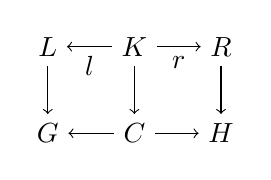
\begin{tikzpicture}[node distance=11mm]
          \node (I) {$K$};
          \node (L) [left of= I] {$L$};
          \node (R) [right of=I] {$R$}; 
          \node (G) [below of=L] {$G$};
          \node (C) [below of=I] {$C$};
          \node (H) [below of=R] {$H$};
        %   \node (T) [left=of $(L)!0.5!(G)$] {$T$};
        %   \draw [->] (L) to  node [label, above] {$c$}  (T);
        %   \draw [->] (G) to  node [label, below] {$\alpha$} (T);
          \draw [->] (I) to node [label, below] {$l$} (L);
          \draw [->] (I) to node [label, below] {$r$} (R);
          \draw [->] (L) to  (G);
          \draw [->] (I) to (C);
          \draw [->] (R) to (H);
          \draw [->] (C) to (G);
          \draw [->] (C) to (H);
        \end{tikzpicture}
      \end{center}
\end{minipage}
   \begin{itemize}
       \item $\operatorname{left}(\Delta)$ is weighable with \(\mathcal{T}\),
       \item $\operatorname{right}(\Delta)$ is bounded above by \(\mathcal{T}\), 
       \item $w(e) \mathop{\succeq} 1_S$ for all $e \mathop{\in} \mathbb{E}$.
   \end{itemize}

   \noindent
  We have:
   \begin{itemize}
       \item $\mu(w_\mathcal{T}(G)) \mathop{\succeq} \mu(w_\mathcal{T}(H))$ if $\rho$ is weakly decreasing,
       \item $\mu(w_\mathcal{T}(G)) \mathop{>} \mu(w_\mathcal{T}(H))\mathop{+}\delta$ if $\rho$ is $\delta$-uniformly or $\delta$-closure decreasing for some $\delta >0$ and $w(e) \mathop{\succeq} 1_S$ for all $e \mathop{\in} \mathbb{E}$.
   \end{itemize}
\end*{}

\begin{proof}
    \label{proof:decreasing_step}
    \noindent For every \( t_K: K \mathop{\rightarrow} T \), we define
$
        S_{t_K} \overset{\operatorname{def}}{=}   
        \underset{\substack{t_C:C \mathop{\rightarrow} T \\
        t_K \mathop{=} h_{KC} \mathop{\star} t_C }}{\mathop{\bigoplus}} 
        w_\mathcal{T}(t_C - h_{KC})  
$.
    
    \noindent For all $t_K: K \mathop{\to} T$ and $X,Y \mathop{\in} S$, the following claims hold:
    \begin{enumerate}[label=(\alph*)] 
        \item \label{s_nz} $S_{t_K} \ne 0_S$ if there is $t_C$ with $ t_K \mathop{=} h_{KC} \mathop{\star} t_C$.  
        \begin{proof}
            By definition of weighted type graph, for all $e \mathop{\in} \mathbb{E}$, we have 
            \begin{flalign}
                w(e) \mathop{\neq} 0_S \label{eq_we_neq_0s1111}
            \end{flalign}
            For every $t_C:C \mathop{\to} T$, we have 
            \begin{flalign*}
                &w_\mathcal{T}(t_C - h_{KC}) \\
               =&\mathop{\bigodot}_{e\in \mathbb{E}} w_e(t_C - h_{KC}) & \text{by Definition~\ref{def:weight_excluding}}\\
               =&\mathop{\bigodot}_{e\in \mathbb{E}} 
                 \mathop{\bigodot}_{\substack{\alpha \mathop{\in} \{- * t_C \mathop{=} e\}\\
                    \alpha \notin \left\{ \iota \mathop{\in} \operatorname{Hom}(X, C)~\middle|~\exists \zeta:X \mathop{\to} K,~\zeta \mathop{\star} h_{KC} \mathop{=} \iota \right\}
                 }
                 } w(e)  & \text{by Definition~\ref{def:weight_excluding_pre}} \\
               \mathop{\neq}&0_S & \text{by \eqref{eq_we_neq_0s1111}, \eqref{eq:prop_neq0_mul_neq0} and Definition~\ref{def:bigodot}}  
            \end{flalign*}

            Therefore, $S_{t_K} \overset{\operatorname{def}}{=}   
            \underset{\substack{t_C:C \mathop{\rightarrow} T \\
            t_K \mathop{=} h_{KC} \mathop{\star} t_C }}{\mathop{\bigoplus}} 
            w_\mathcal{T}(t_C - h_{KC}) \mathop{\neq} 0_S$ if there exists be a morphism such that $t_K \mathop{=} h_{KC} \mathop{\star} t_C$ by \eqref{eq:prop_neq0_plus_neq0}.
            % For every $t_C:C \mathop{\to} T$ such that $t_K \mathop{=} h_{KC} \mathop{\star} t_C$, we have $w_\mathcal{T}(t_C - h_{KC}) \mathop{\neq} 0_S$ by \eqref{eq:prop_neq0_mul_neq0}. 
        \end{proof}
        
        \item \label{s_ge1} $S_{t_K} \mathop{\succeq} 1_S$ if there is $t_C$ with $ t_K \mathop{=} h_{KC} \mathop{\star} t_C$ and $w_\mathcal{T}(e) \mathop{\succeq} 1_S$ for all $e \mathop{\in} \mathbb{E}$,
        \begin{proof}
            By the definition of weighted type graph, for all $e \mathop{\in} \mathbb{E}$, we have $w(e) \mathop{\neq} 0_S$.  
            By assumption, we have $w_\mathcal{T}(e) \mathop{\succeq} 1_S$ for all $e \mathop{\in} \mathbb{E}$. Thus, we have 
            \begin{flalign}
                1_S \mathop{\preceq} w(e) \mathop{\neq} 0_S \label{eq_we_neq_0s_geq1_0}
            \end{flalign}
            By \eqref{eq:prop_neg0_ge1_mul_ge1}, we have
            \begin{flalign}
                1_S \mathop{\preceq} w_\mathcal{T}(t_C - h_{KC}) \label{eq_we_neq_0s_geq1}
            \end{flalign}

            Therefore, $S_{t_K} \overset{\operatorname{def}}{=}   
            \underset{\substack{t_C:C \mathop{\rightarrow} T \\
            t_K \mathop{=} h_{KC} \mathop{\star} t_C }}{\mathop{\bigoplus}} 
            w_\mathcal{T}(t_C - h_{KC}) \mathop{\succeq} 1_S$ if there exists be a morphism such that $t_K \mathop{=} h_{KC} \mathop{\star} t_C$ by \eqref{ax:s1}.
        \end{proof}
        
        % \item \label{claim:le} $Y \mathop{\succeq} X \implies  Y \mathop{\odot} S_{t_K} \mathop{\succeq} X \mathop{\odot} S_{t_K}$
        % \\ by Axiom \eqref{ax:s3}. \todo{to delete: inutile}
         
        \item \label{claim:st} if there exists $t_C$ with $t_K \mathop{=} h_{KC} \mathop{\star} t_C$ then
        $$ \mu(Y) \mathop{>} \mu(X)\mathop{+}\delta  \implies \mu(Y \mathop{\odot} S_{t_K}) \mathop{>} \mu(X \mathop{\odot} S_{t_K})$$
                % $$\left (\exists \alpha \mathop{\geq} \delta.~\mu(Y) \mathop{>} \mu(X)\mathop{+}\alpha \right ) \implies (\mu(Y \mathop{\odot} S_{t_K}) \mathop{>} \mu(X \mathop{\odot} S_{t_K}))$$
        \begin{proof}
           Suppose that there is $t_C$ with $t_K \mathop{=} h_{KC} \mathop{\star} t_C$. We have $S_{t_K} \mathop{\neq} 0_S$ by \ref{s_nz}, and we conclude by \eqref{ax:s4''}.
        \end{proof}
    
        \item \label{claim:sh_{DT}elta} 
        if there exists $t_C$ with $t_K \mathop{=} h_{KC} \mathop{\star} t_C$, and  $w_\mathcal{T}(e) \mathop{\succeq} 1_S$ for all $e \mathop{\in} \mathbb{E}$ then
        % $$\left (\exists \alpha \mathop{\geq} \delta.~\mu(Y) \mathop{>} \mu(X)\mathop{+} \alpha \right ) \implies (\exists \beta \mathop{\geq} \delta. \mu(Y \mathop{\odot} S_{t_K}) \mathop{>} \mu(X \mathop{\odot} S_{t_K}) \mathop{+}\beta)$$
        $$\mu(Y) \mathop{>} \mu(X)\mathop{+} \delta \implies \mu(Y \mathop{\odot} S_{t_K}) \mathop{>} \mu(X \mathop{\odot} S_{t_K}) \mathop{+}\delta $$
        \begin{proof}
            Suppose that there is $t_C$ with $t_K \mathop{=} h_{KC} \mathop{\star} t_C$. We have $1_S \mathop{\preceq} S_{t_K} \mathop{\neq} 0_S$ by \ref{s_nz} and \ref{s_ge1}, and we conclude by \eqref{ax:s4'}. 
        \end{proof}

        \item \label{claim:0} 
        if there is no $t_C$ with $t_K \mathop{=} h_{KC} \mathop{\star} t_C$ then  $S_{t_K} \mathop{=} 0_S$, thus
        $$Y \mathop{\odot} S_{t_K} \mathop{=} 0_S \mathop{=} X \mathop{\odot} S_{t_K} $$
    
        \item \label{claim:exist_st} 
        If there is a context closure $t_L$ for $\rho$ and $T$ in $\mathfrak{F}$ , then, let $t_K \mathop{=} l \mathop{\star} t_L$, we have
        $$ \mu(Y) \mathop{>} \mu(X)\mathop{+}\delta \implies \mu(Y \mathop{\odot} S_{t_K}) \mathop{>} \mu(X \mathop{\odot} S_{t_K})$$
        \begin{proof}
            
       By Definition~\ref{def:context_closure} of context closure, there exists $t_G : G \mathop{\rightarrow} T$ such that 
        \begin{flalign*}
             t_L \mathop{=} h_{LG} \mathop{\star} t_G \tag{1} \label{eq_tl_hlg_tg}
        \end{flalign*}
      i.e. we have the following commutative diagram
     
    \begin{center}
        \begin{tikzpicture}[node distance=11mm]
          \node (I) {$K$};
          \node (L) [left of= I] {$L$};
          \node (R) [right of=I] {$R$};
          \node (G) [below of=L] {$G$};
          \node (C) [below of=I] {$C$};
          \node (H) [below of=R] {$H$};
          \node (T) [left=of $(L)!0.5!(G)$] {$T$};
          \draw [->] (L) to  node [label, above] {$t_L$}  (T);
          \draw [->] (G) to  node [label, below] {$t_G$} (T);
          \draw [->] (I) to node [label, above] {$l$} (L);
          \draw [->] (I) to node [label,above] {$r$} (R);
        %   \draw [->] (L) to node [label, right] {$m$} (G);
        \draw [->] (L) to node [label, right] {} (G);
          \draw [->] (I) to (C);
          \draw [->] (R) to (H);
          \draw [->] (C) to (G);
          \draw [->] (C) to (H);
        \end{tikzpicture}
      \end{center}
    
        Let $t_C \overset{\operatorname{def}}{=} h_{CG} \mathop{\star} t_G$ and $t_K \overset{\operatorname{def}}{=} l \mathop{\star} t_L$. We have\\
        \begin{flalign*}
              t_K  &=  l \mathop{\star} t_L &\text{by definition of $t_K$}
            \\ &=   l \mathop{\star} (h_{LG}  \mathop{\star} t_G) & \text{by~\autoref{eq_tl_hlg_tg}}
            \\ &= (l \mathop{\star} h_{LG}) \mathop{\star} t_G &\text{by associativity }
            \\ &= (h_{KC} \mathop{\star} h_{CG}) \mathop{\star} t_G & \text{by commutative of $\square KLGC$}
            \\ &= h_{KC} \mathop{\star} (h_{CG}  \mathop{\star} t_G) & \text{by associativity}
            \\ & \mathop{=} h_{KC} \mathop{\star} t_C &\text{by definition of $t_C$}
        \end{flalign*}
        and the claim follows from \ref{claim:st}, sinc $t_C$ is a morphism such that $t_K \mathop{=} h_{KC} \mathop{\star} t_C$.
    \end{proof}

        \item \label{claim:exist_sh_{DT}elta} 
        If there is a context closure $t_L$ for $\rho$ and $T$ in $\mathfrak{F}$, and $w_\mathcal{T}(e) \mathop{\succeq} 1_S$ for all $e \mathop{\in} \mathbb{E}$ then, let $t_K \mathop{=} l \mathop{\star} t_L$, we have 
            % $$\left (\exists \alpha \mathop{\geq} \delta. Y \mathop{\succ} X\mathop{+} \alpha \right ) \implies (\exists \beta \mathop{\geq} \delta. Y \mathop{\odot} S_{t_K} \mathop{\succ} X \mathop{\odot} S_{t_K} \mathop{+}\beta)$$
        $$Y \mathop{\succ} X\mathop{+}\delta \implies Y \mathop{\odot} S_{t_K} \mathop{\succ} X \mathop{\odot} S_{t_K} \mathop{+}\delta$$ 
        \begin{proof}
            The proof is analogous to the proof of \ref{claim:exist_st} but with \ref{claim:sh_{DT}elta} instead of \ref{claim:st} in the end.
        \end{proof} 
    \end{enumerate}
    
    \noindent For every \( t_K: K \mathop{\rightarrow} T \), let
    \begin{flalign*}
        \Lambda_{t_K} &\overset{\operatorname{def}}{=}  w_\mathcal{T}(\{l \mathop{\star} - \mathop{=} t_K\})
        \\
        \Omega_{t_K} &\overset{\operatorname{def}}{=}  w_\mathcal{T}(\{r \mathop{\star} - \mathop{=} t_K\})
    \end{flalign*}
  By~\autoref{lem_4d13}, we have 
        \begin{flalign*} 
            w_\mathcal{T}(G) &=
                \underset{\substack{t_K: K \mathop{\rightarrow} T}}{\mathop{\bigoplus}}     \ \
            (S_{t_K} \mathop{\odot} \Lambda_{t_K})
              \\
            w_\mathcal{T}(H) &\mathop{\preceq}
            \underset{\substack{t_K: K \mathop{\rightarrow} T}}{\mathop{\bigoplus}}     \ \
                (S_{t_K} \mathop{\odot} \Omega_{t_K})
        \end{flalign*}

    \noindent We complete the proof with a analysis by cases:
    \begin{enumerate}
        \item  If $\rho$ is weakly decreasing, then, by Definition~\ref{def:decreasing_rule} of weakly decreasing rule, we have $\Lambda_{t_K} \mathop{\geq} \Omega_{t_K}$
        for every $t_K: K \mathop{\rightarrow} T$. 
        By \eqref{ax:s3}, for every  $ t_K : K \mathop{\rightarrow} T$, we have 
                \begin{flalign*} 
                    S_{t_K} \mathop{\odot} \Lambda_{t_K} \mathop{\succeq} S_{t_K} \mathop{\odot} \Omega_{t_K} \tag{NE} \label{steps:weightC:ge} 
                \end{flalign*}
        Thus, we have $w_\mathcal{T}(G) \mathop{\succeq} w_\mathcal{T}(H)$, from \eqref {ax:s1}.
        % \item
        %     If $\rho$ is $\delta$-uniformly decreasing for some $\delta \mathop{\in} \mathbb{R}_{>0}$, then, by Definition~\ref{def:decreasing_rule} of $\delta$-uniformly decreasing rule,
        %     for all $t_K : K \mathop{\to} T$, we have 
        %                     \begin{itemize}                                
        %                         \item $\exists \alpha \mathop{\geq} \delta.~\mu(\Lambda_{t_K}) \mathop{>} \mu(\Omega_{t_K})\mathop{+}\alpha$, or
        %                         \item $\{l \mathop{\star} - \mathop{=} t_K\} \mathop{=} \emptyset \mathop{=} \{r \mathop{\star} - \mathop{=} t_K\}$
        %                     \end{itemize}
        %     From \ref{claim:st} and \ref{claim:0}, for every \( t_K: K \mathop{\rightarrow} T \), we have
        %     \begin{enumerate}[label=(\roman*)]
        %         \item $S_{t_K} \mathop{\odot} \Lambda_{t_K} \mathop{=} 0_S \mathop{=}  S_{t_K} \mathop{\odot} \Omega_{t_K}$, or        
        %         \item  \label{it:strict} $ \mu(\Lambda_{t_K} \mathop{\odot} S_{t_K}) \mathop{>}  \mu(S_{t_K} \mathop{\odot} \Omega_{t_K})$
        %     \end{enumerate}
        %     To establish $ \mu(w_\mathcal{T}(G)) \mathop{>} \mu(w_\mathcal{T}(H))$, using \eqref{ax:s2}, 
        %     it suffices to show that we have case~\ref{it:strict} for some $t_K : K \mathop{\to} T$.
        %     This follows from \ref{claim:exist_st} since we have a context closure for $\rho$ and $\mathcal{T}$, by assumption.
        \item  
            Suppose that $\rho$ is $\delta$-uniformly decreasing for $\delta \mathop{\in} \mathbb{R}_{>0}$, and $w_\mathcal{T}(e) \mathop{\succeq} 1$ for all $e \mathop{\in} \mathbb{E}$. By Definition~\ref{def:decreasing_rule} of $\delta$-uniformly decreasing rule,
            for all $t_K : K \mathop{\to} T$, we have  
                            \begin{itemize}                                
                                \item $\mu(\Lambda_{t_K}) \mathop{>} \mu(\Omega_{t_K})\mathop{+}\delta$,
                                % $\exists \alpha \mathop{\geq} \delta  .~\mu(\Lambda_{t_K}) \mathop{>} \mu(\Omega_{t_K})\mathop{+}\alpha$, 
                                 or
                                \item $\{l \mathop{\star} - \mathop{=} t_K\} \mathop{=} \emptyset \mathop{=} \{r \mathop{\star} - \mathop{=} t_K\}$
                            \end{itemize}
            From \ref{claim:sh_{DT}elta} and \ref{claim:0}, for every \( t_K: K \mathop{\rightarrow} T \), we obtain
            \begin{enumerate}[label=(\roman*)]
                \item $S_{t_K} \mathop{\odot} \Lambda_{t_K} \mathop{=} 0_S \mathop{=}  S_{t_K} \mathop{\odot} \Omega_{t_K}$, or
                \item  \label{it:strich_{DT}elta}  $\mu(\Lambda_{t_K} \mathop{\odot} S_{t_K}) \mathop{>} \mu(\Omega_{t_K} \mathop{\odot} S_{t_K})\mathop{+}\delta$
                % $\exists \beta \mathop{\geq} \delta  .\  \mu(\Lambda_{t_K} \mathop{\odot} S_{t_K}) \mathop{>} \mu(\Omega_{t_K} \mathop{\odot} S_{t_K})\mathop{+}\beta$
            \end{enumerate}
            To establish $ \mu(w_\mathcal{T}(G)) \mathop{>} \mu(w_\mathcal{T}(H))\mathop{+}\delta$, using \eqref{ax:s2'}, 
            it suffices to show that we have case~\ref{it:strich_{DT}elta} for some $t_K : K \mathop{\to} T$.
            This follows from \ref{claim:exist_sh_{DT}elta} since we have a context closure for $\rho$ and $\mathcal{T}$ by assumption.
            % \item
            % If $\rho$ is $\delta$-closure decreasing, 
            % then it is also weakly decreasing and we obtain \eqref{steps:weightC:ge} for every $t_K : K \mathop{\to} T$.
            % Since the semiring is strictly ordered museurable, it suffices to show that there exists some $t_K : K \mathop{\to} T$ such that
            % \begin{align}
            %    \mu( S_{t_K} \mathop{\odot} \Lambda_{t_K})  \mathop{\succ} \mu(S_{t_K} \mathop{\odot} \Omega_{t_K})
            %   \tag{$\star$} \label{steps:weightC:gt}
            % \end{align}
            % in order to conclude $\mu(w_\mathcal{T}(G)) \mathop{>} \mu(w_\mathcal{T}(H))$ by Equation~\eqref{ax:s5}.
            % By Definition~\ref{def:decreasing_rule}, there is a context closure $t_L$ for $\rho$ and $T$, and 
            % % $\exists \delta' \mathop{\geq} \delta  .\  \Lambda_{t_K} \mathop{>} \Omega_{t_K}\mathop{+}\delta'$
            % $\mu(\Lambda_{t_K}) \mathop{>} \mu(\Omega_{t_K})\mathop{+}\delta$
            % for $t_K \mathop{=} l \mathop{\star} t_L$. Thus, we obtain  Equation~\eqref{steps:weightC:gt} by~\ref{claim:exist_st}.
        \item
            If $\rho$ is $\delta$-closure decreasing, and $w_\mathcal{T}(e) \mathop{\succeq} 1$ for all $e \mathop{\in} \mathbb{E}$ then it is also weakly decreasing and we obtain \eqref{steps:weightC:ge} for every $t_K : K \mathop{\to} T$.
            Since the semiring is a strictly monotonic museurable semiring,  by~\autoref{ax:s2'} and \eqref{ax:s5'}, it suffices to show that there exists some $t_K : K \mathop{\to} T$ such that 
            \begin{align}
                % \exists \alpha \mathop{\geq} \delta.~
                \mu(S_{t_K} \mathop{\odot} \Lambda_{t_K}) \mathop{>} \mu(S_{t_K} \mathop{\odot} \Omega_{t_K})\mathop{+}
                \delta
                % \alpha
              \tag{$\star\star$}\label{steps:weightC:gh_{DT}elta}
            \end{align}
            in order to conclude $ \mu(w_\mathcal{T}(G)) \mathop{>} \mu(w_\mathcal{T}(H))\mathop{+}\delta$.
            There is a context closure $t_L$ for $\rho$ and $T$, and
            $\mu(\Lambda_{t_K}) \mathop{>} \mu(\Omega_{t_K})\mathop{+}\delta$
            % $\exists \delta' \mathop{\geq} \delta  .\  \Lambda_{t_K} \mathop{>} \Omega_{t_K}\mathop{+}\delta'$
            for $t_K \mathop{=} l \mathop{\star} t_L$. Thus, we obtain Equation~\eqref{steps:weightC:gh_{DT}elta} by~\ref{claim:exist_sh_{DT}elta}.
    \end{enumerate}
    \end{proof} 
    
    

\noindent\begin*{\textbf{\autoref{thm:termination_grs}}}
Let $\mathcal{A}$ and $\mathcal{B}$ be sets of DPO rewriting rules, $\mathcal{T} \mathop{=} (T,\mathbb{E}, (S, \mathop{\oplus}, \mathop{\odot}, 0_S, 1_S, \prec, \mu), w)$ a finitary weighted type graph and $\mathfrak{F}$ a DPO rewriting framework such that

\begin{enumerate}[label=\roman*)]
   \item\label{thm1:hyp3} $w(e) \mathop{\succeq} 1_S$ for all $e \mathop{\in} \mathbb{E}$,
   % \item\label{thm1:hyp4} $\{s \mathop{\in} S\mid 1_S \leq s \mathop{\neq} 0_S\} \mathop{\subseteq} \mathbb{R}_{>0}$ 
   % \item\label{thm1:hyp4} for all $x \mathop{\in} S$, if $ 1_S \mathop{\preceq} x \mathop{\neq} 0_S$ then $\mu(x) \mathop{\geq} \mu(1_S)$ and $\mu(x) \mathop{\in} \mathbb{R}$,
   \item\label{thm1:hyp4} for all $x \mathop{\in} S$, if $ 1_S \mathop{\preceq} x \mathop{\neq} 0_S$ then $\mu(x) \mathop{\geq} \mu(1_S)$ and $\mu(x) \mathop{\in} \mathbb{R}$,
   \item for every rule $\rho \mathop{\in} (\mathcal{A }\mathop{\cup} \mathcal{B })$ and every double pushout diagram  
   $\Delta \mathop{\in} \mathfrak{F}(\rho)$ 
   \begin{itemize}
       \item \(\operatorname{left}(\Delta)\) is weighable with \(\mathcal{T}\),
       \item \(\operatorname{right}(\Delta)\) is bounded above by \(\mathcal{T}\). 
   \end{itemize}
\end{enumerate}       

\noindent If the following conditions hold:
\begin{enumerate}
   \item there exists $\delta >0$ such that either every $\rho \mathop{\in} \mathcal{A}$ is $\delta$-uniformly, or every $\rho \mathop{\in} \mathcal{A}$ is $\delta$-closure decreasing,
   \item every rule $\rho \mathop{\in} \mathcal{B}$ is weakly decreasing,
\end{enumerate}
then $\mathop{\Rightarrow}_{\mathcal{A},\mathfrak{F}}$ is \textbf{terminating} relative to $\mathop{\Rightarrow}_{\mathcal{B},\mathfrak{F}}$.
\end*{}


\begin{proof} 
    \label{proof_termination_grs}
    From the definition of weighted type graph, we have 
    $$\text{for all}~e\in\mathbb{E}, w(e) \mathop{\neq} 0_S$$ 
    From ssumption \eqref{thm1:hyp3}, we have 
    $$\text{for all}~e\in\mathbb{E},1_S \mathop{\preceq} w(e)$$
    Therefore, we have 
    \begin{flalign}
        \text{for all}~e\in\mathbb{E},1_S \mathop{\preceq} w(e)\mathop{\neq} 0_S \label{thm_eq_we_neq0_geq1}
    \end{flalign} 
    Let $G$ be a graph admitting a match of a DPO rewriting rule. We have 
    \begin{flalign*}
        w_\mathcal{T}(G) &\overset{\operatorname{def}}{=} 
            \underset{h \mathop{\in} \operatorname{Hom}(G,T)}{\mathop{\bigoplus}}  w_\mathcal{T}(h) \\
        & \overset{\operatorname{def}}{=} 
        \underset{h \mathop{\in} \operatorname{Hom}(G,T)}{\mathop{\bigoplus}} 
            \left ( \underset{e \mathop{\in} \mathbb{E}}{\mathop{\bigodot}} 
            \left(  
                \underset{\alpha \mathop{\in} \{- \mathop{\star} h \mathop{=} e\}}{\mathop{\bigodot}}w(e) 
            \right)
            \right )\\
    \end{flalign*} 
    By~\autoref{thm_eq_we_neq0_geq1},~\autoref{prop_endrullis_2d7}, {def:bigodot} and $1_S \mathop{\neq} 0_S$, for every $h \mathop{\in} \operatorname{Hom}(G,T)$, we have
    \begin{flalign}
        1_S \mathop{\preceq} 
        \underset{e \mathop{\in} \mathbb{E}}{\mathop{\bigodot}} 
                \left(  
                    \underset{\alpha \mathop{\in} \{- \mathop{\star} h \mathop{=} e\}}{\mathop{\bigodot}}w(e) 
                \right) 
        \mathop{\neq} 0_S
    \end{flalign}
    Since $G$ be a graph admitting a match of a DPO rewriting rule, by~\autoref{prop_endrullis_2d7} and \eqref{ax:s0}, we have $$1_S \mathop{\preceq} w_\mathcal{T}(G) \mathop{\neq} 0_S$$
    % By~\autoref{prop_endrullis_2d7} and \eqref{ax:s0}, we have 
    % $$\forall G\in\mathcal{C}_0, (\exists H\in \mathcal{C}_0. G \mathop{\Rightarrow}_\mathcal{R} H) \mathop{\rightarrow} (1_S \mathop{\preceq} w_\mathcal{T}(G) \mathop{\neq} 0_S)$$
    By Assumption \eqref{thm1:hyp4}, we have 
    % $$\forall G\in\mathcal{C}_0, (\exists H\in \mathcal{C}_0. G \mathop{\Rightarrow}_\mathcal{R} H) \mathop{\rightarrow} (\mu(w_\mathcal{T}(G)) \mathop{\geq} \mu(1_S))$$
      $$\mu(w_\mathcal{T}(G)) \mathop{\geq} \mu(1_S)$$
 
    % Let $G \mathop{\in} \mathcal{C}_0$ be an object. By Assumption \ref{thm1:hyp4}, we have $\mu(w_\mathcal{T}(G)) \mathop{\in} \mathbb{R}$ and $\mu(w_\mathcal{T}(G)) \mathop{\geq} \mu(1_S)$.

    By~\autoref{lem:decreasing_step}, every rewriting step with rules in $\mathcal{A}$ strictly decreases the weight by at least $\delta$ and no rewriting step with rules in $\mathcal{B}$ increases the weight.
    Consequently, there is no infinite rewriting sequence with an infinite rewriting steps with rules in $\mathcal{A}$ from $G$.
\end{proof}

% \noindent\begin*{\textbf{\autoref{thm:termination_gls}}}
%     Let $\mathfrak{F}$ be a DPO rewriting framework, $\mathcal{A}$ and $\mathcal{B}$ sets of graph relabelling rules and $\mathcal{T} \mathop{=} (T,\mathbb{E}, S, w)$ a finitary weighted type graph such that 
%     \begin{itemize}
%             \item for all $x \mathop{\in} S$, if $x \mathop{\neq} 0_S$ then $\mu(x) \mathop{\in} \mathbb{R}$.
%     \end{itemize}

% \noindent If the following conditions hold
%     \begin{itemize}
%     \item every rule $\rho \mathop{\in} \mathcal{B}$ is weakly decreasing,
%     \item for every $\rho \mathop{\in} \mathcal{A}$, $\rho$ is $0$-uniform or $0$-closure decreasing,
%     \end{itemize}
%     then $\mathcal{A }$ is \textbf{terminating} relative to $\mathcal{B }$.
% \end*{}

% \begin{proof} 
%     By the definition, we have 
%     $$\forall e \mathop{\in} \mathbb{E}. w(e) \mathop{\neq} 0_S$$

%     By~\autoref{prop_endrullis_2d7}, we have 
%         $$\forall G\in\mathcal{C}_0, (\exists H\in \mathcal{C}_0. G \mathop{\Rightarrow}_\mathcal{R} H) \mathop{\rightarrow}  w_\mathcal{T}(G) \mathop{\neq} 0_S$$

%     By assumption, we have 
%      $$\forall G\in\mathcal{C}_0, (\exists H\in \mathcal{C}_0. G \mathop{\Rightarrow}_\mathcal{R} H) \mathop{\rightarrow}  \mu(w_\mathcal{T}(G)) \mathop{\in} \mathcal{R}$$

%     Let $G \mathop{\in} \mathcal{C}_0$ be an object. We have $w_\mathcal{T}(G) \mathop{\in} \mathbb{R}$.

%     By~\autoref{lem:decreasing_step}, every rewriting step with rules in $\mathcal{A}$ strictly decreases the weight by at least $\delta$ and no rewriting step with rules in $\mathcal{R}$ increases the weight.

%     Consequently, there is no infinite rewriting sequence with an infinite rewriting steps with rules in $\mathcal{A}$ from some $G \mathop{\in} \mathcal{C}$, because otherwise there would be an infinite number of accessible objects from $G$ which contradicts the fact that with a given finite unlabeled graph, there are only a finite number of possible labeled graphs for the set of label is finite.
% \end{proof}
    